% BANKS-SOURCE: pdf=38 print=28 kind=section id=3.5
\subsection{Legendre's trees}

% BANKS-SOURCE: pdf=38 print=28 kind=prose
The graphical assertions of the previous two paragraphs were that the Legendre
transform relation

% BANKS-SOURCE: pdf=38 print=28 kind=equation id=3.35
\begin{equation}
W[J]=\int\dd^D x\,\phi(x)J(x)+\Gamma[\phi]
\label{eq:3.35}
\end{equation}

(where $\phi(x)$ is identified with $\delta W/\delta J(x)$ and $J(x)$ with $-\delta\Gamma/\delta\phi(x)$) generates an
expansion of the (connected) Green functions obtained from the expansion of $W$ in
terms of tree diagrams whose vertices are the 1PI Green functions and whose branches
are the full propagator

% BANKS-SOURCE: pdf=39 print=29 kind=display
\[
\frac{\delta^2W}{\delta J(x)\delta J(y)}.
\]

In leading order in the semi-classical expansion we have $\Gamma=S/g^2$.
The proof of this relation is simple. We start from the obvious identity

% BANKS-SOURCE: pdf=39 print=29 kind=display
\[
\frac{\delta^2W}{\delta J(x)\delta J(y)}
=\frac{\delta\phi(y)}{\delta J(x)}
=\left(\frac{\delta J(y)}{\delta\phi(x)}\right)^{-1}
=-\frac{\delta^2\Gamma}{\delta\phi(x)\delta\phi(y)}.
\]

The inverse in the second equality is meant in the sense of integral operators,

% BANKS-SOURCE: pdf=39 print=29 kind=display
\[
\int\dd^D z\,K(x,z)K^{-1}(z,y)=\delta^D(x-y),
\]

which is the continuous analog of matrix inversion. We write this as $W_2=-\Gamma_2^{-1}$, where
$\Gamma_2$ is the integral operator made from the 1PI two-point function.
Differentiate this identity with respect to $J(z)$,

% BANKS-SOURCE: pdf=39 print=29 kind=equation id=3.36
\begin{equation}
\frac{\delta^3W}{\delta J(x)\delta J(y)\delta J(z)}=-\frac{\delta\Gamma_2^{-1}(x,y)}{\delta J(z)},
\label{eq:3.36}
\end{equation}

and use the continuous analog of the matrix differentiation formula $\dd K^{-1}=-K^{-1}\dd K K^{-1}$ to write this as

% BANKS-SOURCE: pdf=39 print=29 kind=equation id=3.37
\begin{equation}
W_3(x,y,z)=\int\dd^D w_1\,\dd^D w_2\,W_2(x,w_1)W_2(y,w_2)\frac{\delta\Gamma_2(w_1,w_2)}{\delta J(z)}.
\label{eq:3.37}
\end{equation}

Using the chain rule for differentiation and the relation $\phi=\delta W/\delta J$, this becomes

% BANKS-SOURCE: pdf=39 print=29 kind=equation id=3.38
\begin{equation}
W_3(x,y,z)=\int\dd^D w_1\,\dd^D w_2\,\dd^D w_3\,W_2(x,w_1)W_2(y,w_2)W_2(z,w_3)\Gamma_3(w_1,w_2,w_3).
\label{eq:3.38}
\end{equation}

This is the formula implied by the three-point position-space Feynman diagram of
Figure~\ref{fig:3.1}.
It is now all over except for the shouting, which mathematicians call induction. When
we differentiate $W_3$ w.r.t. $J(s)$, the derivatives act either on the propagators or on $\Gamma_3$.
The latter contribution gives the first term in the four-point diagram of Figure~\ref{fig:3.1}. For
the former, we simply rerun the previous derivation to get the second four-point term.
Similarly, for $W_n$, either differentiation acts on the $\Gamma_k$, with $3\leq k\leq n$, and generates
$\Gamma_{k+1}$ and an extra external $W_2$ leg, or it acts on one of the propagators, adding an
extra three-point vertex and external propagator. In words, $W_n$ is generated from all
possible tree diagrams.

This result is very powerful. Below we will show that the exact momentum-space
two-point function, $W_2(p)$ (when $J=0$ the two-point function is translation-invariant
and its Fourier transform depends only on one variable), has a pole at the mass of
any stable particle that can be created from the vacuum by the quantum field $\phi$. The

% BANKS-SOURCE: pdf=40 print=30 kind=figure id=3.1
\begin{figure}[htbp]
  \centering
  \resizebox{0.97\textwidth}{!}{%
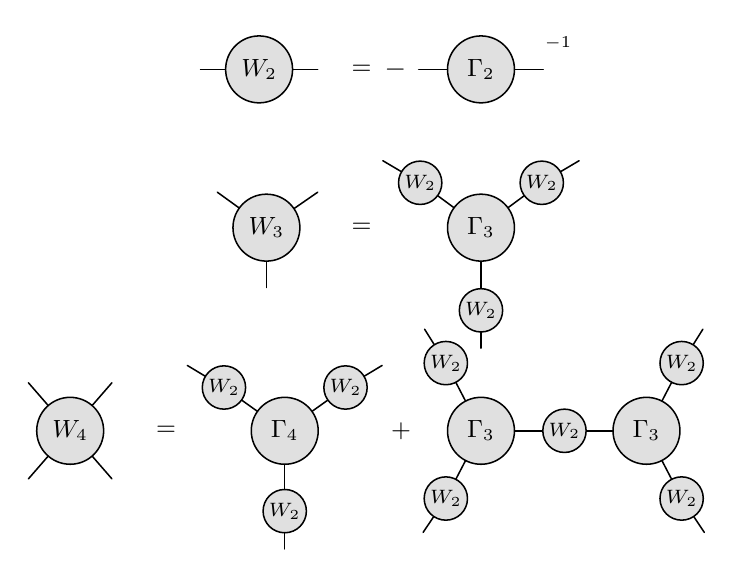
\begin{tikzpicture}[x=0.93cm,y=1cm,xshift=0.28cm,baseline=(current bounding box.center),
  line cap=round,line join=round,
  every node/.style={font=\small},
  L/.style={line width=.55pt},
  v/.style={draw,line width=.55pt,circle,fill=black!12,minimum size=8.5mm,inner sep=0pt},
  e/.style={draw,line width=.55pt,circle,fill=black!12,minimum size=5.5mm,inner sep=0pt}]

  %% ---- row 1:  --(W_2)--  =  - --(Gamma_2)--^{-1}
  \draw[L] (1.78,4.59) -- (3.38,4.59);
  \draw[L] (4.76,4.59) -- (6.46,4.59);

  %% ---- row 2:  W_3  =  Gamma_3 dressed by three W_2 on its legs
  % W_3 legs
  \draw[L] (2.68,2.58) -- (2.01,3.03);
  \draw[L] (2.68,2.58) -- (3.38,3.03);
  \draw[L] (2.68,2.58) -- (2.68,1.82);
  % Gamma_3 legs, each carrying a W_2 which continues to an external stub
  \draw[L] (5.61,2.58) -- (4.78,3.15) -- (4.27,3.43);
  \draw[L] (5.61,2.58) -- (6.44,3.15) -- (6.95,3.43);
  \draw[L] (5.61,2.58) -- (5.61,1.53) -- (5.61,1.05);

  %% ---- row 3:  W_4  =  Gamma_4 term  +  Gamma_3--W_2--Gamma_3 term
  % W_4 legs
  \draw[L] (0,0) -- (-0.57,0.61);
  \draw[L] (0,0) -- (0.57,0.61);
  \draw[L] (0,0) -- (-0.57,-0.61);
  \draw[L] (0,0) -- (0.57,-0.61);
  % Gamma_4 term (drawn in the source with three dressed legs)
  \draw[L] (2.93,0) -- (2.10,0.55) -- (1.60,0.83);
  \draw[L] (2.93,0) -- (3.76,0.55) -- (4.26,0.83);
  \draw[L] (2.93,0) -- (2.93,-1.02) -- (2.93,-1.50);
  % Gamma_3 -- W_2 -- Gamma_3 term
  \draw[L] (5.61,0) -- (7.87,0);
  \draw[L] (5.61,0) -- (5.13,0.86) -- (4.84,1.29);
  \draw[L] (5.61,0) -- (5.13,-0.86) -- (4.82,-1.29);
  \draw[L] (7.87,0) -- (8.35,0.86) -- (8.64,1.29);
  \draw[L] (7.87,0) -- (8.35,-0.86) -- (8.66,-1.29);

  %% ---- blobs (drawn last so they mask the leg stubs underneath)
  % row 1
  \node[v] at (2.58,4.59) {$W_2$};
  \node    at (3.98,4.59) {$=$};
  \node[font=\normalsize] at (4.44,4.59) {$-$};
  \node[v] at (5.61,4.59) {$\Gamma_2$};
  \node    at (6.66,4.92) {$\scriptstyle -1$};
  % row 2
  \node[v] at (2.68,2.58) {$W_3$};
  \node    at (3.98,2.58) {$=$};
  \node[v] at (5.61,2.58) {$\Gamma_3$};
  \node[e] at (4.78,3.15) {\scriptsize$W_2$};
  \node[e] at (6.44,3.15) {\scriptsize$W_2$};
  \node[e] at (5.61,1.53) {\scriptsize$W_2$};
  % row 3
  \node[v] at (0,0) {$W_4$};
  \node    at (1.31,0) {$=$};
  \node[v] at (2.93,0) {$\Gamma_4$};
  \node[e] at (2.10,0.55) {\scriptsize$W_2$};
  \node[e] at (3.76,0.55) {\scriptsize$W_2$};
  \node[e] at (2.93,-1.02) {\scriptsize$W_2$};
  \node    at (4.52,0) {$+$};
  \node[v] at (5.61,0) {$\Gamma_3$};
  \node[e] at (6.75,0) {\scriptsize$W_2$};
  \node[v] at (7.87,0) {$\Gamma_3$};
  \node[e] at (5.13,0.86) {\scriptsize$W_2$};
  \node[e] at (5.13,-0.86) {\scriptsize$W_2$};
  \node[e] at (8.35,0.86) {\scriptsize$W_2$};
  \node[e] at (8.35,-0.86) {\scriptsize$W_2$};
\end{tikzpicture}%
}

  \caption{Legendre transform $W[J]=\Gamma[\phi]+\int\dd^D x\,\phi J$ makes trees.}
  \label{fig:3.1}
\end{figure}
\BanksImplicitHook{I-CH03-014}
